%----------------------------------------------------------------------------------------
%	PACKAGES AND DOCUMENT CONFIGURATIONS
%----------------------------------------------------------------------------------------

\documentclass{article}

\usepackage{lmodern}
\usepackage{multirow}
\usepackage{subcaption}
\usepackage{graphicx} % Required for the inclusion of images
\graphicspath{{images/}}

\setlength\parindent{0pt} % Removes all indentation from paragraphs

\renewcommand{\labelenumi}{\alph{enumi}.} % Make numbering in the enumerate environment by letter rather than number (e.g. section 6)

%\usepackage{times} % Uncomment to use the Times New Roman font

%----------------------------------------------------------------------------------------
%	DOCUMENT INFORMATION
%----------------------------------------------------------------------------------------

\title{A* Search Implementation for Blocks World} % Title

\author{Matthew Grogan} % Author name

\date{\today} % Date for the report

\begin{document}

\maketitle % Insert the title, author and date

% If you wish to include an abstract, uncomment the lines below
% \begin{abstract}
% Abstract text
% \end{abstract}

%----------------------------------------------------------------------------------------
%	SECTION 1
%----------------------------------------------------------------------------------------

\section{Overview}

We have been tasked with implementing an A* search solution to the Blocksworld
problem.In this version of Blocksworld, we must arrange a finite number of blocks on a finite
number of stacks such that the blocks are placed in ascending order on the first
stack. To facilitate ordering, each block is given a label such as A or B and
each stack is numbered. The last block on any given stack can be moved to the
last position on any other stack. For simplicity's sake, I have replaced letters 
A, B, etc. with numbers 1, 2, etc. 

%----------------------------------------------------------------------------------------
%	SECTION 2
%----------------------------------------------------------------------------------------

\section{Implementation}
\subsection{A*}

My implementation of A* and Blocksworld is written in C++. I use three
classes:
\begin{enumerate}
    \item A state class containg stack and block information as well as member
	functions for moving and evaluating current block configurations.
    \item A node class which contains a parent pointer, a state class variable,
	and a path cost estimate.
    \item An A* search class containing a frontier priority queue, visited list,
	and the search algorithm.
\end{enumerate}

\subsection{Heuristic}
\subsubsection{Description}

The heuristic I have constructed is presented below.
We start our move counter with the number of blocks in the problem. We check the
first stack and decrement the counter for each block in place. This gives us a
simple number-of-blocks-out-of-place heuristic. But we know that each block out
of place in the first stack must be moved again, so we increment count in this
case. Next we check the other stacks. For each block in the stack, we look at
each of the blocks underneath it. If the current block is the larger of the
comparison, we know that it must be moved to free up the burried block and we
increment the move count.

\hspace*{1cm}\textsc{Set count = \# of blocks}\\
\hspace*{1cm}\textsc{\underline{For} each block in stack one, do:}\\
\hspace*{2cm}\textsc{\underline{if} block is in position, decrement count}\\
\hspace*{2cm}\textsc{\underline{else}, increment count}\\
\hspace*{1cm}\textsc{\underline{For} each stack past stack one, do:}\\
\hspace*{2cm}\textsc{\underline{For} each block in this stack, do:}\\
\hspace*{3cm}\textsc{\underline{For} each sub-block under this top-block,do:}\\
\hspace*{4cm}\textsc{\underline{if} sub-block < top-block, increment count}\\
\hspace*{1cm}\textsc{return count}



\subsubsection{Admissibility}

This heuristic is not admissible. Consider a case such as\\
\textsc{1 :}\\
\textsc{2 :}\\
\textsc{3 : A B C}\\
In this case, the heuristic returns a value of 6 when the optimal solution is
in only 5 moves. Even in this case, the heuristic guides us towards the correct
solution by encouraging proper ordering and avoidance of the first row for
incorrect blocks. The above case is not particularly likely and for smaller
values (e.g. 3 stacks and 5 blocks). It becomes more prominant with larger
numbers of blocks in proportion to stacks as this results in generally lasrger
stacks.

%----------------------------------------------------------------------------------------
%	SECTION 3
%----------------------------------------------------------------------------------------

\section{Results}

The solution performs quite well in comparison to the simple
blocks-out-of-place baseline. This can be seen in Figure~\ref{fig:comparison}
and in Table~\ref{tab:comparison}. The solution is also reasonably scalable,
generally finding solutions within 10,000 search steps for problems in the
3-stack-8-block to 5-stack-11-block range. Beyond this, performance is largly
dependent on a favorable starting configuration. Some performance metrics can be
found in Figure~\ref{fig:heuristic} and Table~\ref{tab:heuristic}.

%----------------------------------------------------------------------------------------
%	SECTION 4
%----------------------------------------------------------------------------------------

\section{Discussion}

The heuristic worked as expected in that it drastically improved search time
over an uninformed approach. A consequence of my implementation is that paths
with smaller (B=2, C=3, ...) blocks on top are strongly favored. As a result of
this and the fact that my heuristic is not admissible, performance breaks down 
with a small number of large stacks and non-optimal solutions can be produced.
However, good results are still produced within the belt of 3 stacks and 8
blocks, 5 stacks and 11 blocks, and 10 stacks with 15 blocks. With these ranges,
the queue can grow to a substantial size. The size of the queue is related to the
efficiency of the search, obviously, but specifically the number of stacks and
the number of search steps. The branching factor increases by a factor of
around the number of stacks and search iterations multiplies this.
When the number of stacks is increased, as in Figure~\ref{fig:heuristic} the 
heuristic performs better in terms of search time. This is due to the fact that 
more available stacks allow blocks to be rearranged without creating conflicts
for another block.\\\\ 
One possible heuristic that I considered was one which
considered the relationships between blocks and when what at first appears to be
a conflict actually lies along the optimal solution path. That direction seemed
to be an endless expansion of corner cases and the relatively simple heuristic
which I settled on generally outperformed a more complicated approaches. My
heuristic could, however, be stregnthened by 'improving' admissibility. This would
involve accounting for the case outlined above when the blocks are arranged in
nearly reverse order on non-goal stacks. Since my heuristic punishes large
stacks, immediately succesful moves may be overlooked in the interest of
reducing a stack. This is highly troublesome on problems with high block to
stack ratios. As can be seen in
Table~\ref{tab:heuristic}, the relative error becomes negative for large numbers
of blocks indicating a consistent overestimate of cost. Interestingly,
underestimating heuristics which I worked on were outperformed by the
inadmissible heuristic. I believe that to effectively improve performance, I
might need to restructure my formulation of the problem space, adding relational
attributes for blocks rather than treating them as numbers in arrays.

\section{Figures and Tables}

\begin{table}[h]
\resizebox{\columnwidth}{!}{
    \begin{tabular}{ @{}|l|l|l|l|l|l|l|l|@{} }
    \hline
    \multicolumn{8}{ |c| }{Heuristic Comparison with 3 Stacks} \\ \hline
    Number of Blocks & H & Depth & Steps & QL & Error & Samples & Failures \\ \hline
    \multirow{2}{*}{3} & H1 & 3.91 & 18.995 & 57.334 & 0.263 & 1000 & 0 \\ 
		    & H2 & 3.855 & 6.042 & 21.202 & 0.011 & 1000 & 0 \\ \hline
    \multirow{2}{*}{4} & H1 & 5.91 & 162.833 & 541.627 & 0.347 & 1000 & 0 \\ 
		    & H2 & 5.934 & 22.787 & 84.101 & 0.022 & 1000 & 0 \\ \hline
    \multirow{2}{*}{5} & H1 & 7.811 & 1636.75 & 5903.22 & 0.38 & 289 & 4 \\ 
		    & H2 & 8.143 & 105.792 & 410.92 & 0.029 & 1000 & 0 \\ \hline
    \end{tabular}
}
\caption{Comparison of a range of parameters. H1 indicates the out-of-place
    heuristic and H2 is outlined above}
\label{tab:comparison}
\end{table}

\begin{table}[h]
\resizebox{\columnwidth}{!}{
    \begin{tabular}{ @{}|l|l|l|l|l|l|l|l|@{} }
    \hline
    \multicolumn{8}{ |c| }{Performance Metrics} \\ \hline
    \# Stacks & \# Blocks & Depth & Steps & QL & Error & Samples & Failures \\ \hline
    3 & 3 & 3.855 & 6.042 & 21.202 & 0.011 & 1000 & 0 \\ \hline
    3 & 4 & 5.934 & 22.787 & 84.101 & 0.022 & 1000 & 0 \\ \hline
    3 & 5 & 8.143 & 105.792 & 410.92 & 0.029 & 1000 & 0 \\ \hline
    4 & 5 & 6.926 & 47.614 & 346.335 &0.008 & 1000 & 0 \\ \hline
    5 & 5 & 6.405 & 39.675 & 449.017 & 0.001 & 1000 & 0 \\ \hline
    5 & 10 & 15.185 & 689.407 & 10863.44 & -0.012 & 30 & 4\\ \hline
    6 & 5 & 6.199 & 42.819 & 651.251 & -4.76E-05 & 1000 & 0 \\ \hline
    10 & 10 & 12.552 & 132.862 & 7910.103 & -0.034 & 60 & 2\\ \hline
    10 & 15 & 9.965 & 158.827 & 11239.24 & -0.023 & 30 & 1\\ \hline
    \end{tabular}
}
\caption{Comparison of a range of performance metrics for hueristic}
\label{tab:heuristic}
\end{table}

\begin{figure}[h]
    \centering
    \begin{subfigure}{\linewidth}
	\centering
	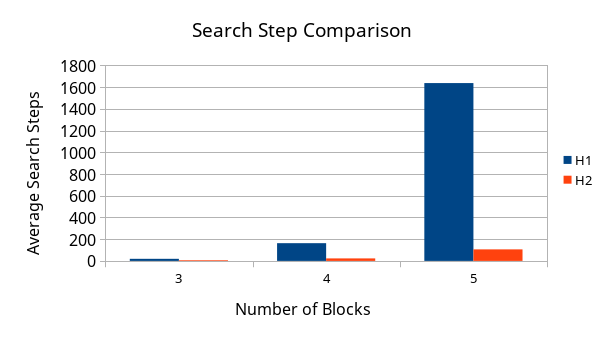
\includegraphics[width=.65\linewidth]{H1vsH2_AvgSteps.png}\hfill
	\caption{}
    \end{subfigure}\par\medskip
    \begin{subfigure}{\linewidth}
	\centering
	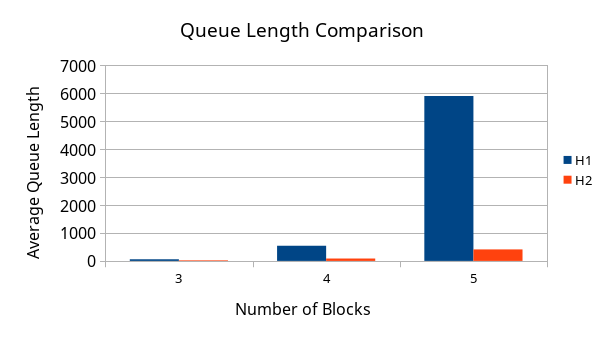
\includegraphics[width=.65\linewidth]{H1vsH2_AvgQL.png}\hfill
	\caption{}
    \end{subfigure}\par\medskip
    \begin{subfigure}{\linewidth}
	\centering
	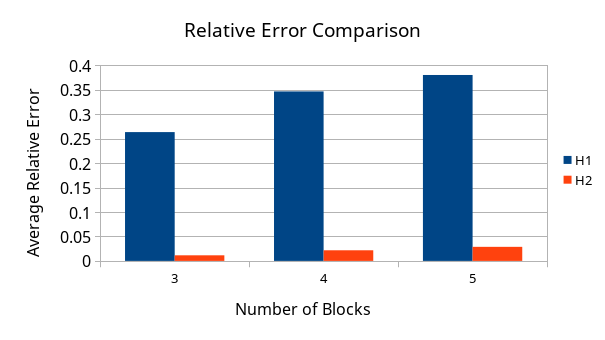
\includegraphics[width=.65\linewidth]{H1vsH2_AvgRelErr.png}\hfill
	\caption{}
    \end{subfigure}
    \caption{A comparison of the performance of two heuristics for three
    stacks: H1 is blocks-out-of-place, H2 is that outlined above }
    \label{fig:comparison}
\end{figure}

\begin{figure}[h]
    \centering
    \begin{subfigure}{\linewidth}
	\centering
	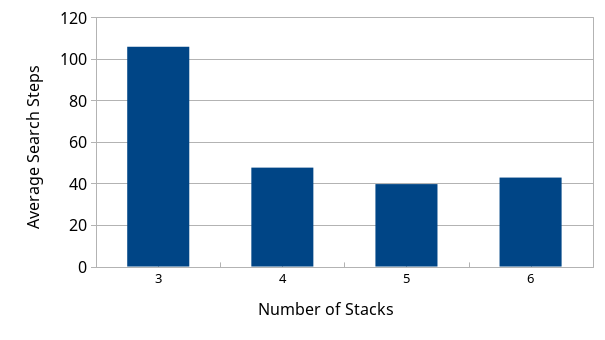
\includegraphics[width=.65\linewidth]{H2_AvgStepsVsStacks.png}\hfill
	\caption{Number of search steps}
    \end{subfigure}\par\medskip
    \begin{subfigure}{\linewidth}
	\centering
	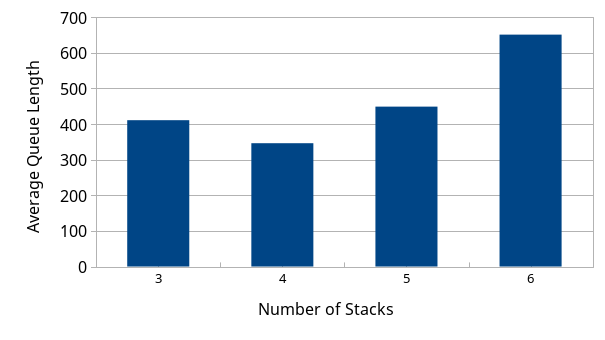
\includegraphics[width=.65\linewidth]{H2_AvgQLVsStacks.png}\hfill
	\caption{Queue length}
    \end{subfigure}\par\medskip
    \begin{subfigure}{\linewidth}
	\centering
	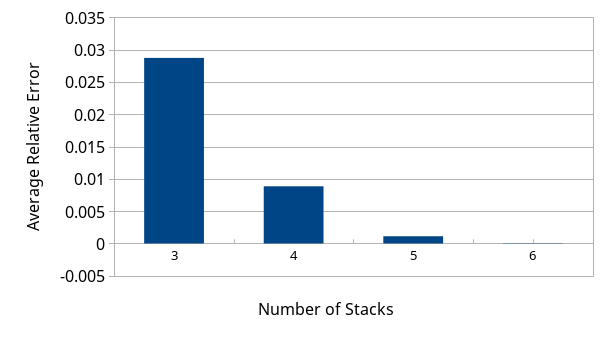
\includegraphics[width=.65\linewidth]{H2_AvgRelErrVsStacks.png}\hfill
	\caption{Relative error}
    \end{subfigure}
    \caption{Performance of heuristic with five blocks and varying stacks}
    \label{fig:heuristic}
\end{figure}

\end{document}
